\documentclass[11pt,]{article}
\usepackage{lmodern}
\usepackage{amssymb,amsmath}
\usepackage{ifxetex,ifluatex}
\usepackage{fixltx2e} % provides \textsubscript
\ifnum 0\ifxetex 1\fi\ifluatex 1\fi=0 % if pdftex
  \usepackage[T1]{fontenc}
  \usepackage[utf8]{inputenc}
\else % if luatex or xelatex
  \ifxetex
    \usepackage{mathspec}
  \else
    \usepackage{fontspec}
  \fi
  \defaultfontfeatures{Ligatures=TeX,Scale=MatchLowercase}
\fi
% use upquote if available, for straight quotes in verbatim environments
\IfFileExists{upquote.sty}{\usepackage{upquote}}{}
% use microtype if available
\IfFileExists{microtype.sty}{%
\usepackage{microtype}
\UseMicrotypeSet[protrusion]{basicmath} % disable protrusion for tt fonts
}{}
\usepackage[margin=0.79in]{geometry}
\usepackage{hyperref}
\hypersetup{unicode=true,
            pdftitle={Test},
            pdfauthor={AlistairGJ},
            pdfborder={0 0 0},
            breaklinks=true}
\urlstyle{same}  % don't use monospace font for urls
\usepackage{color}
\usepackage{fancyvrb}
\newcommand{\VerbBar}{|}
\newcommand{\VERB}{\Verb[commandchars=\\\{\}]}
\DefineVerbatimEnvironment{Highlighting}{Verbatim}{commandchars=\\\{\}}
% Add ',fontsize=\small' for more characters per line
\usepackage{framed}
\definecolor{shadecolor}{RGB}{255,255,255}
\newenvironment{Shaded}{\begin{snugshade}}{\end{snugshade}}
\newcommand{\AlertTok}[1]{\textcolor[rgb]{0.75,0.01,0.01}{\textbf{\colorbox[rgb]{0.97,0.90,0.90}{#1}}}}
\newcommand{\AnnotationTok}[1]{\textcolor[rgb]{0.79,0.38,0.79}{#1}}
\newcommand{\AttributeTok}[1]{\textcolor[rgb]{0.00,0.34,0.68}{#1}}
\newcommand{\BaseNTok}[1]{\textcolor[rgb]{0.69,0.50,0.00}{#1}}
\newcommand{\BuiltInTok}[1]{\textcolor[rgb]{0.39,0.29,0.61}{\textbf{#1}}}
\newcommand{\CharTok}[1]{\textcolor[rgb]{0.57,0.30,0.62}{#1}}
\newcommand{\CommentTok}[1]{\textcolor[rgb]{0.54,0.53,0.53}{#1}}
\newcommand{\CommentVarTok}[1]{\textcolor[rgb]{0.00,0.58,1.00}{#1}}
\newcommand{\ConstantTok}[1]{\textcolor[rgb]{0.67,0.33,0.00}{#1}}
\newcommand{\ControlFlowTok}[1]{\textcolor[rgb]{0.12,0.11,0.11}{\textbf{#1}}}
\newcommand{\DataTypeTok}[1]{\textcolor[rgb]{0.00,0.34,0.68}{#1}}
\newcommand{\DecValTok}[1]{\textcolor[rgb]{0.69,0.50,0.00}{#1}}
\newcommand{\DocumentationTok}[1]{\textcolor[rgb]{0.38,0.47,0.50}{#1}}
\newcommand{\ErrorTok}[1]{\textcolor[rgb]{0.75,0.01,0.01}{\underline{#1}}}
\newcommand{\ExtensionTok}[1]{\textcolor[rgb]{0.00,0.58,1.00}{\textbf{#1}}}
\newcommand{\FloatTok}[1]{\textcolor[rgb]{0.69,0.50,0.00}{#1}}
\newcommand{\FunctionTok}[1]{\textcolor[rgb]{0.39,0.29,0.61}{#1}}
\newcommand{\ImportTok}[1]{\textcolor[rgb]{1.00,0.33,0.00}{#1}}
\newcommand{\InformationTok}[1]{\textcolor[rgb]{0.69,0.50,0.00}{#1}}
\newcommand{\KeywordTok}[1]{\textcolor[rgb]{0.12,0.11,0.11}{\textbf{#1}}}
\newcommand{\NormalTok}[1]{\textcolor[rgb]{0.12,0.11,0.11}{#1}}
\newcommand{\OperatorTok}[1]{\textcolor[rgb]{0.12,0.11,0.11}{#1}}
\newcommand{\OtherTok}[1]{\textcolor[rgb]{0.00,0.43,0.16}{#1}}
\newcommand{\PreprocessorTok}[1]{\textcolor[rgb]{0.00,0.43,0.16}{#1}}
\newcommand{\RegionMarkerTok}[1]{\textcolor[rgb]{0.00,0.34,0.68}{\colorbox[rgb]{0.88,0.91,0.97}{#1}}}
\newcommand{\SpecialCharTok}[1]{\textcolor[rgb]{0.24,0.68,0.91}{#1}}
\newcommand{\SpecialStringTok}[1]{\textcolor[rgb]{1.00,0.33,0.00}{#1}}
\newcommand{\StringTok}[1]{\textcolor[rgb]{0.75,0.01,0.01}{#1}}
\newcommand{\VariableTok}[1]{\textcolor[rgb]{0.00,0.34,0.68}{#1}}
\newcommand{\VerbatimStringTok}[1]{\textcolor[rgb]{0.75,0.01,0.01}{#1}}
\newcommand{\WarningTok}[1]{\textcolor[rgb]{0.75,0.01,0.01}{#1}}
\usepackage{graphicx,grffile}
\makeatletter
\def\maxwidth{\ifdim\Gin@nat@width>\linewidth\linewidth\else\Gin@nat@width\fi}
\def\maxheight{\ifdim\Gin@nat@height>\textheight\textheight\else\Gin@nat@height\fi}
\makeatother
% Scale images if necessary, so that they will not overflow the page
% margins by default, and it is still possible to overwrite the defaults
% using explicit options in \includegraphics[width, height, ...]{}
\setkeys{Gin}{width=\maxwidth,height=\maxheight,keepaspectratio}
\IfFileExists{parskip.sty}{%
\usepackage{parskip}
}{% else
\setlength{\parindent}{0pt}
\setlength{\parskip}{6pt plus 2pt minus 1pt}
}
\setlength{\emergencystretch}{3em}  % prevent overfull lines
\providecommand{\tightlist}{%
  \setlength{\itemsep}{0pt}\setlength{\parskip}{0pt}}
\setcounter{secnumdepth}{5}
% Redefines (sub)paragraphs to behave more like sections
\ifx\paragraph\undefined\else
\let\oldparagraph\paragraph
\renewcommand{\paragraph}[1]{\oldparagraph{#1}\mbox{}}
\fi
\ifx\subparagraph\undefined\else
\let\oldsubparagraph\subparagraph
\renewcommand{\subparagraph}[1]{\oldsubparagraph{#1}\mbox{}}
\fi

%%% Use protect on footnotes to avoid problems with footnotes in titles
\let\rmarkdownfootnote\footnote%
\def\footnote{\protect\rmarkdownfootnote}

%%% Change title format to be more compact
\usepackage{titling}

% Create subtitle command for use in maketitle
\providecommand{\subtitle}[1]{
  \posttitle{
    \begin{center}\large#1\end{center}
    }
}

\setlength{\droptitle}{-2em}

  \title{Test}
    \pretitle{\vspace{\droptitle}\centering\huge}
  \posttitle{\par}
    \author{AlistairGJ}
    \preauthor{\centering\large\emph}
  \postauthor{\par}
      \predate{\centering\large\emph}
  \postdate{\par}
    \date{06/11/2019}

\usepackage{booktabs}
\usepackage{longtable}
\usepackage{array}
\usepackage{multirow}
\usepackage[table]{xcolor}
\usepackage{wrapfig}
\usepackage{float}
\usepackage{colortbl}
\usepackage{pdflscape}
\usepackage{tabu}
\usepackage{threeparttable}
\usepackage{threeparttablex}
\usepackage[normalem]{ulem}
\usepackage{makecell}

\usepackage{booktabs} \usepackage{longtable} \usepackage{array} \usepackage{multirow} \usepackage[table]{xcolor} \usepackage{wrapfig} \usepackage{float} \floatplacement{figure}{H} \usepackage{caption, setspace} \captionsetup[figure]{font={stretch=1,scriptsize}} \captionsetup[table]{font={stretch=1,scriptsize}}

\begin{document}
\maketitle

SPELL CHECK

\hypertarget{table-of-contents}{%
\section{Table of Contents}\label{table-of-contents}}

\begin{enumerate}
\def\labelenumi{\arabic{enumi}.}
\tightlist
\item
  \protect\hyperlink{Background}{Background}
\item
  \protect\hyperlink{Dataux5cux2520Preprocessingux5cux2520ux5cux26ux5cux2520Visualisation}{Data
  Preprocessing \& Visualisation} 2.1
  \protect\hyperlink{Importingux5cux2520ux5cux26ux5cux2520Preprocessingux5cux2520theux5cux2520Activitiesux5cux2520Metaux5cux2520Data}{Importing
  \& Preprocessing the Activities Meta Data}
\item
  \protect\hyperlink{third-example}{Third Example}
\item
  \protect\hyperlink{fourth-examplehttpwwwfourthexamplecom}{Fourth
  Example}
\end{enumerate}

CB!!! citation\_package: biblatex TABLES + FIGURES CB
\url{http://www.ctex.org/documents/packages/float/caption.pdf}
\url{https://stackoverflow.com/questions/32634274/knit-hooksset-and-opts-chunkset}
\url{https://github.com/yihui/knitr/issues/1102}
\url{https://alanarnholt.github.io/GeneralStatistics/rmarkdown/FormattingTables.html}
knit\_hooks\$set(crop = hook\_pdfcrop)

\begin{Shaded}
\begin{Highlighting}[]
\CommentTok{# eval=FALSE, }
\ImportTok{import}\NormalTok{ numpy }\ImportTok{as}\NormalTok{ np}
\ImportTok{import}\NormalTok{ pandas }\ImportTok{as}\NormalTok{ pd}
\ImportTok{import}\NormalTok{ json}
\NormalTok{PATH }\OperatorTok{=} \StringTok{'/Users/alistairgj/Documents/GitHub/IoT_ResearchProject/IoT_November'}
\end{Highlighting}
\end{Shaded}

\pagebreak

\hypertarget{background}{%
\section{Background}\label{background}}

\hypertarget{introduction}{%
\subsection{Introduction}\label{introduction}}

\hypertarget{mankind-technology-development}{%
\subsubsection{Mankind, Technology \&
Development}\label{mankind-technology-development}}

Since the inception of the first home computers in the late 1970's
(Press, 1993), modern society has become utterly dependent on and
indeed, inexorably bound to digital technology. The rapid and widespread
adoption of computational technology has led to the fastest rate of
societal and economic development our species has ever experienced. One
of the most salient manifestations of technical progress has been the
widespread availability and adoption of Information and Communications
Technology (ICT), including the rise of the global network of networks
known as the Internet.

\begin{figure}[H]

{\centering 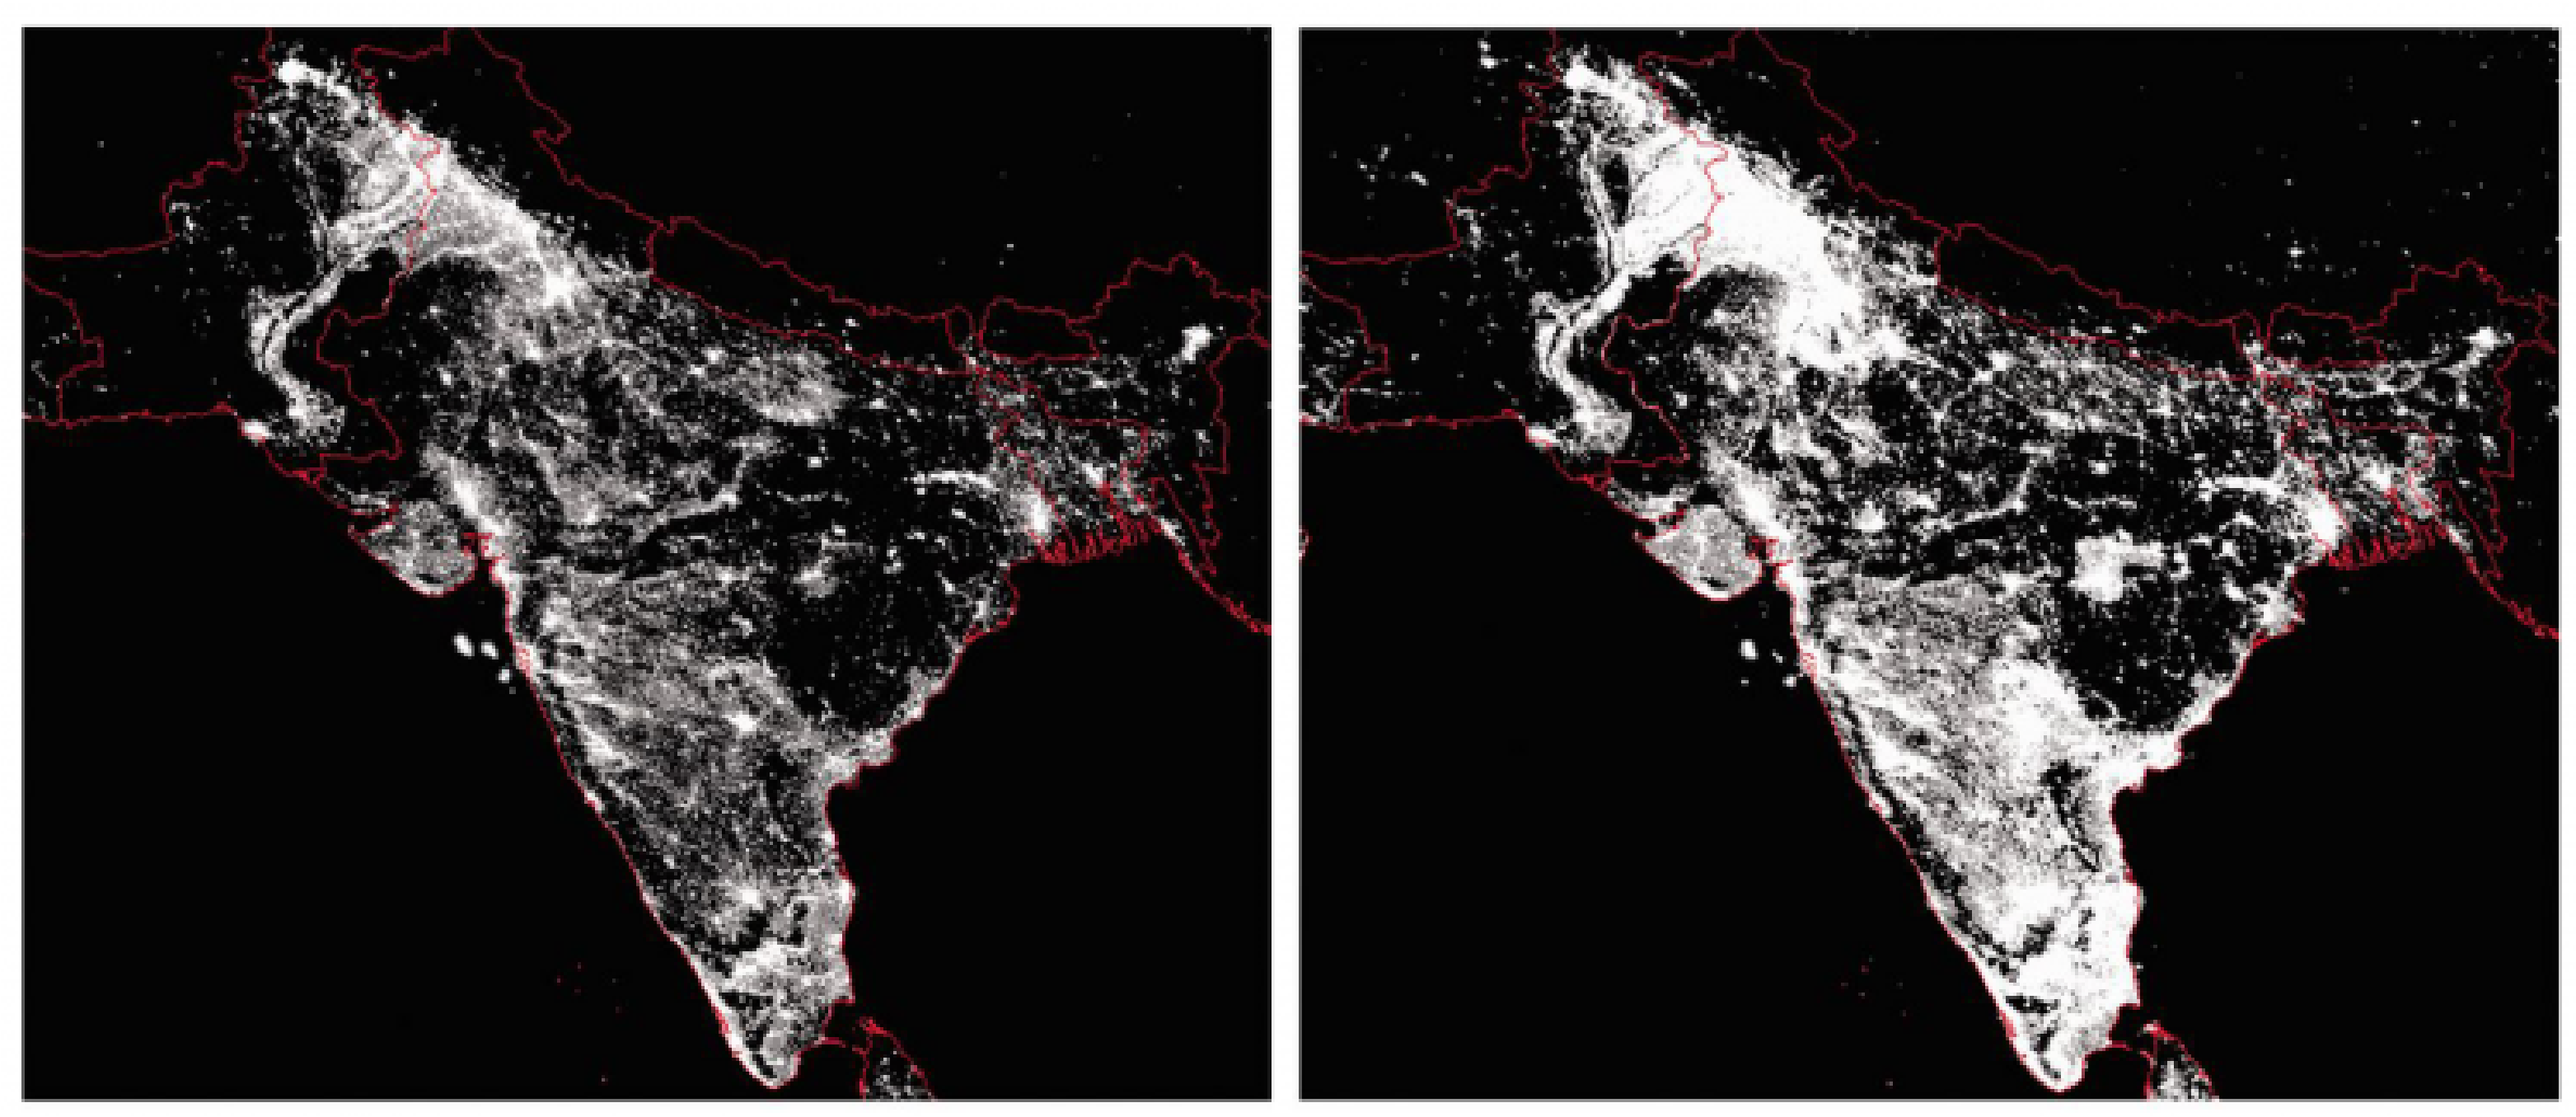
\includegraphics[width=0.6\linewidth]{/Users/alistairgj/Documents/GitHub/IoT_ResearchProject/IoT_November/images/satelliteImages} 

}

\caption{Satellite images of South Asia by night. Left (South Asia in 1994) Right (South Asia in 2010). Images are taken from Maxim Pinkovskiy and Xavier Sala-i-Martin (2016) - Lights, Camera ... Income! Illuminating the National Accounts-Household Surveys Debate. The Quarterly Journal of Economics.}\label{fig:satelliteImagesAsia}
\end{figure}

\begin{figure}[H]

{\centering 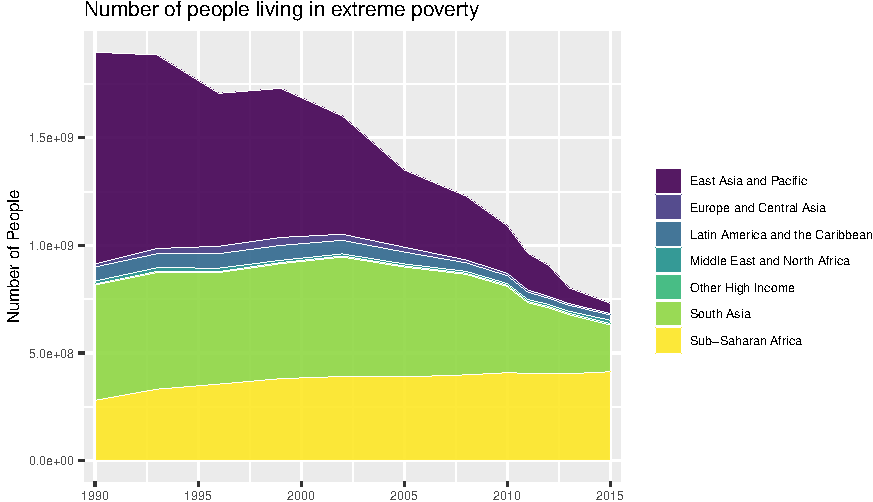
\includegraphics{MD_Final_files/figure-latex/globalPovertyPlot-1} 

}

\caption{ADD TEXT, Source: Our World in Data}\label{fig:globalPovertyPlot}
\end{figure}

\hypertarget{the-rise-and-rise-of-the-world-wide-web}{%
\subsubsection{The Rise and Rise of the World Wide
Web}\label{the-rise-and-rise-of-the-world-wide-web}}

According to the International Telecommunication Union (ITU) 2015 ICTs
figures, Internet penetration has grown from just over 400 millions
users (6 per cent of global population) in 2000 to 3.2 billion users in
2015 (43 per cent of global population), which includes around 2 billion
users from developing countries (Dutta et al., 2015). ICTs bring a broad
range of benefits and are recognised as a key to eradicating poverty and
unemployment. They enable and facilitate the building a people-centred,
inclusive and development-oriented Information Society, where everyone
can create, access, utilize and share information and knowledge. This
enables individuals, communities and peoples to achieve their full
potential in promoting their sustainable development and improving their
quality of life (``Information and communication technologies (ICTs)
\textbar{} Poverty Eradication,'' n.d.).

In addition to a rapidly growing internet user-base both in the
developing and developed world, the nature of internet usage has
fundamentally changed. Once the purview of academics, engineers and
computer scientists sending tiny packets of information back and forth,
there are now some 2.5 quintillion bytes of data created each day by all
manner of users, industry and sensors to name a few (``Data Never Sleeps
5.0 \textbar{} Domo,'' n.d.)

\begin{figure}[H]

{\centering 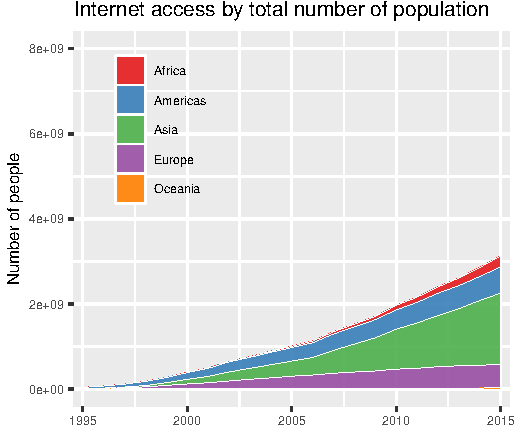
\includegraphics{MD_Final_files/figure-latex/internetAccessPlot-1} 

}

\caption{ADD TEXT}\label{fig:internetAccessPlot}
\end{figure}

\hypertarget{forging-a-new-technological-paradigm}{%
\subsubsection{Forging a New Technological
Paradigm}\label{forging-a-new-technological-paradigm}}

Such rapid and widespread internet adoption has created a seemingly
insatiable demand for exponentially greater computational power and
digital storage capacity. This has led to a new and utterly ubiquitous
technological paradigm; Cloud Computing. Cloud Computing is succinctly
defined as; The practice of using a network of remote servers hosted on
the Internet to store, manage, and process data, rather than a local
server or a personal computer
(\url{https://www.dictionary.com/browse/cloud-computing}).

As with the initial rise and widespread implementation of the internet,
Cloud Computing itself acts as a facilitator for new technologies. One
such example being the Internet of Things (IoT) paradigm. The Internet
of Things can be surmised as the extension of the Internet and the Web
into the physical realm, by means of the widespread deployment of
spatially distributed devices with embedded identification, sensing
and/or actuation capabilities (Daniele Miorandi, 2012). The Internet of
Things (IoT) paradigm enables physical devices to connect and exchange
information, and also allows objects to be sensed or controlled remotely
through the internet (Bing Huang, 2018). IoT devices allow objects to be
sensed or controlled remotely through the Internet (Luigi Atzori, 2010).
IoT thus represents a convergence of real-world objects and digital
objects into a unified cyber-physical system.

\hypertarget{the-bigger-picture}{%
\subsubsection{The Bigger Picture}\label{the-bigger-picture}}

Considering again the bigger picture of societal benefit, Figure X,
shows that the benefits of technological deployment have been widely
adopted and exploited. However, the success of modern human society is
not without consequence. All of the benefits our society has enjoyed
from the development, production and deployment of technology, has
required vast amounts of energy. This energy has, since the industrial
revolution, primarily been derived from the burning of fossil fuels
(REF). The International Panel on Climate Change (IPCC) notes finds that
Human activities are estimated to have caused approximately 1.0°C of
global warming above pre-industrial levels, with a likely range of 0.8°C
to 1.2°C. Global warming is likely to reach 1.5°C between 2030 and 2052
if it continues to increase at the current rate (Intergovernmental Panel
on Climate Change, 2018).

Climate change poses an existential threat to modern human civilisation,
with warming of between 1.5°C and 2°C predicted to cause increases in
mean temperature in most land and ocean regions, hot extremes in most
inhabited regions, heavy precipitation changes including drought and
precipitation deficits in some regions. Additionally, increases in ocean
temperature as well as associated increases in ocean acidity and
decreases in ocean oxygen levels are projected to reduce risks to marine
biodiversity, fisheries, and ecosystems, and their functions and
services to humans. Taken together, these effects will lead to risks of
the health, livelihoods, food security, water supply, human security,
and economic growth of mankind.

\begin{figure}[H]

{\centering 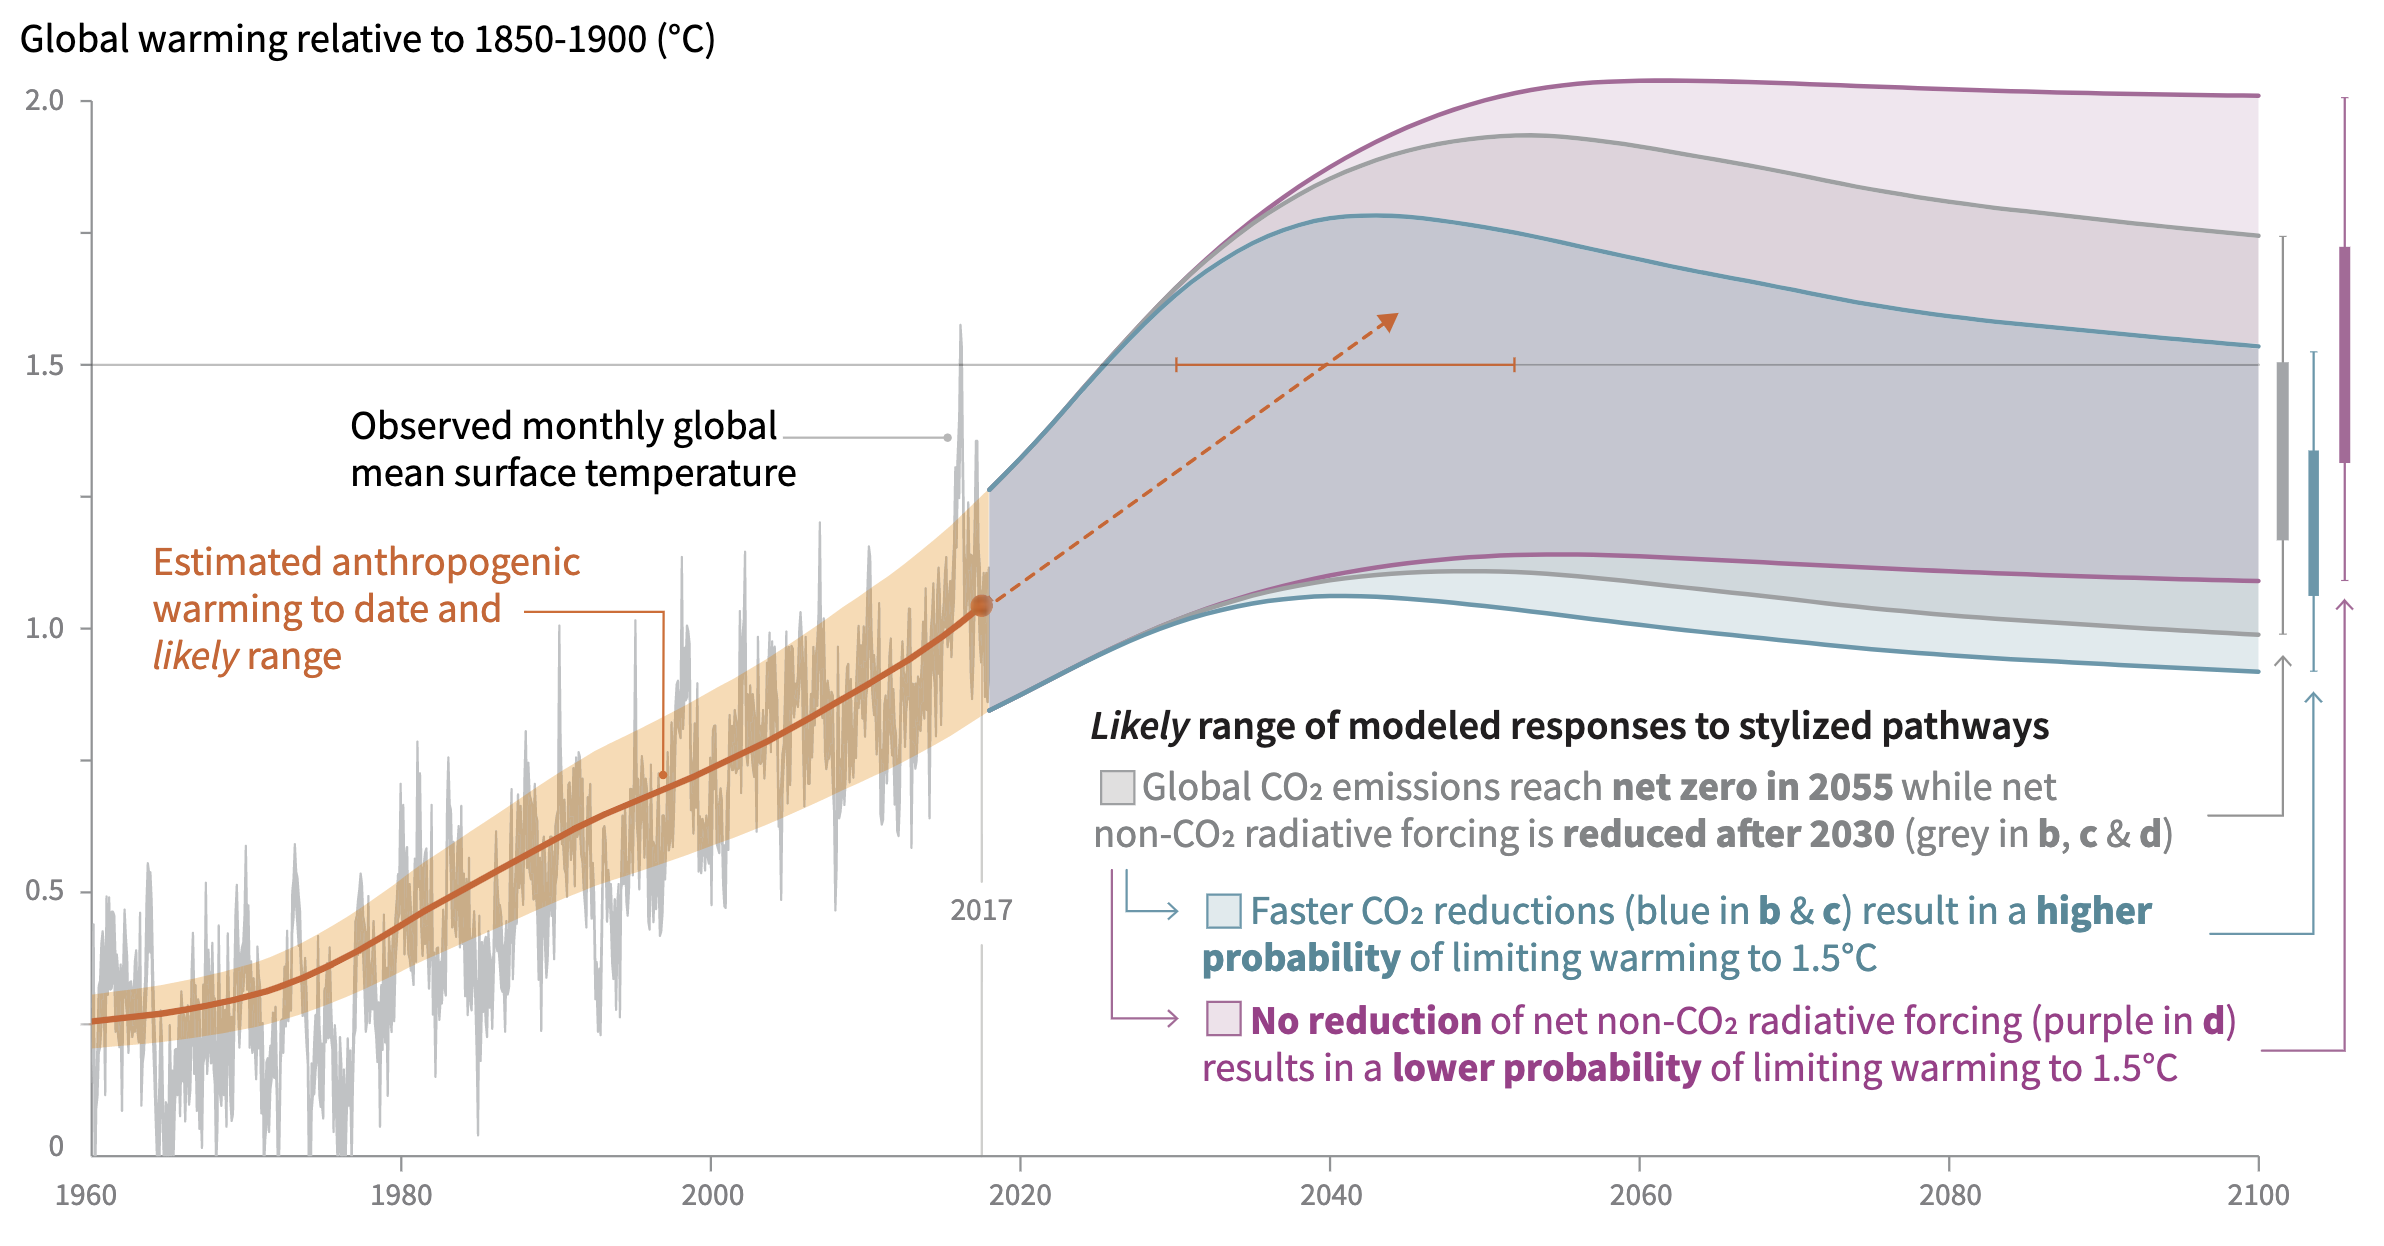
\includegraphics[width=1\linewidth]{/Users/alistairgj/Documents/GitHub/IoT_ResearchProject/IoT_November/images/warmingTrend} 

}

\caption{CAPTION}\label{fig:warmingTrend}
\end{figure}

It is therefore imperative moving forward as a species that all steps
are be taken to mitigate the emission of greenhouse gases and abate the
advance of anthropomorphic climate change. The scale of the challenge is
such that technology itself will prove critical in effectively
combatting this existential threat to civilisation. When considering
energy consumption, the industrial sector (including the non-combusted
use of fuels) currently consumes around half of all global energy and
feedstock fuels, with residential and commercial buildings (29\%) and
transport (21\%) accounting for the remainder
(\url{https://www.bp.com/en/global/corporate/energy-economics/energy-outlook/demand-by-sector.html}).

\hypertarget{optimizing-global-energy-usage-complete}{%
\subsubsection{Optimizing Global Energy Usage
COMPLETE}\label{optimizing-global-energy-usage-complete}}

With residential and commercial buildings accounting for 29\% of energy
demand globally (REF). A qualitative assessment of figures X Y and Z
show that our increased energy consumption has coincided with our
staggering global achievements, including lifting millions out of
poverty blah blah blah. We have more development we use more energy, but
we have more development we are better off in all ways. We ALSO have
more internet connectivity. It therefore stands that the key to
continues human prosperity is to de-couple energy demand growth from
economic growth. Clearly economic prosperity is a direct contributing
factor to human prosperity in general. One such avenue for reduced
energy consumption is the optimization of existing services, utilities,
and so on with respect to the timing, manner and BLAH of their energy
consumption.

\pagebreak

\hypertarget{data-preprocessing-visualisation}{%
\section{Data Preprocessing \&
Visualisation}\label{data-preprocessing-visualisation}}

\hypertarget{importing-preprocessing-the-activities-meta-data}{%
\subsection{Importing \& Preprocessing the Activities Meta
Data}\label{importing-preprocessing-the-activities-meta-data}}

The dataset \texttt{S1Activities.csv} was imported into the interactive
development environment. These data contains a tabulated summary of
Heading, Category, Subcategory and a corresponding code. After
importation, the dataset has dimensionality of {[}3, 33{]}, with
\texttt{Heading}, \texttt{Category} \& \texttt{Subcategory} present as
non-null objects, as seen in Table \ref{tab:S1ActivitiesData} below. The
attribute \texttt{Code} (which codefies the unique set of Heading,
Category) was imported as an index value. At this time, the activities
data will not be kept in it's native state and will not be subject to
preprocessing.

\rowcolors{2}{gray!6}{white}
\begin{table}[!h]

\caption{\label{tab:TAB_S1ActivitiesData}The S1 activities dataset}
\centering
\fontsize{8}{10}\selectfont
\begin{tabular}[t]{llll}
\hiderowcolors
\toprule
  & Heading & Category & Subcategory\\
\midrule
\showrowcolors
1 & Employment related & Employment work at home & Work at home\\
5 & Employment related & Travel employment & Going out to work\\
10 & Personal needs & Eating & Eating\\
15 & Personal needs & Personal hygiene & Toileting\\
20 & Personal needs & Personal hygiene & Bathing\\
\bottomrule
\end{tabular}
\end{table}
\rowcolors{2}{white}{white}

\hypertarget{importing-preprocessing-the-sensor-meta-data}{%
\subsection{Importing \& Preprocessing the Sensor Meta
Data}\label{importing-preprocessing-the-sensor-meta-data}}

The dataset \texttt{S1sensors.csv} was imported into the interactive
development environment. These data contains a tabulated values for
Sensor ID, Room and Sensor Activity Type, with no header row present in
the original dataset. After importation, the dataset has dimensionality
of {[}3, 76{]}, with header 0, 1 \& 2 corresponding to SensorID, Room \&
Sensor Activity Type, respectively, as seen in Table
\ref{tab:TAB_sensorData}. All attributes are nominal, and were imported
as dtype str, accordingly. Attribute attribute 1 \& 2 contain degenerate
values (e.g., Bathroom \& Light Switch). This will be addressed in the
subsequent data preprocessing. The preprocessing of the sensor data is a
critical step in our analysis. Careful consideration of the data,
including the presence of duplicates. This is because if we dont have a
sufficient understanding of where and why duplicates exist, we will not
be able to satisfactorarily preprocess them. Failure to do so we mean
that there is potentail degeneracy in our source dataset, leading to
unknown issues with our downstream analysis.

\rowcolors{2}{gray!6}{white}
\begin{table}[!h]

\caption{\label{tab:TAB_sensorData}The S1 sensor meta data}
\centering
\fontsize{8}{10}\selectfont
\begin{tabular}[t]{lll}
\hiderowcolors
\toprule
0 & 1 & 2\\
\midrule
\showrowcolors
100 & Bathroom & Toilet Flush\\
101 & Bathroom & Light switch\\
104 & Foyer & Light switch\\
105 & Kitchen & Light switch\\
106 & Kitchen & Burner\\
\bottomrule
\end{tabular}
\end{table}
\rowcolors{2}{white}{white}

Column {[}1{]} \& Column {[}2{]} of the sensor data will be
concatenated, whitespace will be removed, all text will be cast to
lowercase and a final whitespace strip will be performed. The python
script \texttt{S1sensorsPreprocessing.py} is run perform several
preprocessing steps in these data. The script concatenates the
attributes \texttt{dsS1Sensors{[}1{]}} and \texttt{dsS1Sensors{[}2{]}},
with an underscore. Whitespace is then stripped and all string values
are coerced to lowercase. This newly created attribute is then added to
the dataframe, as seen below (REF). Additionally, the attributes
\texttt{0}, \texttt{1} \& \texttt{2} are renamed \texttt{subActNum},
\texttt{room} \& \texttt{activity}, respectively.

\begin{itemize}
\tightlist
\item
  Data types
\item
  IF a sub-act requires electricity
\end{itemize}

\rowcolors{2}{gray!6}{white}
\begin{table}[!h]

\caption{\label{tab:TAB_sensorDataProcessed}The first iteration of processed S1 sensor meta data}
\centering
\fontsize{8}{10}\selectfont
\begin{tabular}[t]{llll}
\hiderowcolors
\toprule
subActNum & room & activity & concat\\
\midrule
\showrowcolors
100 & Bathroom & Toilet Flush & bathroom\_toiletflush\\
101 & Bathroom & Light switch & bathroom\_lightswitch\\
104 & Foyer & Light switch & foyer\_lightswitch\\
105 & Kitchen & Light switch & kitchen\_lightswitch\\
106 & Kitchen & Burner & kitchen\_burner\\
\addlinespace
107 & Living room & Light switch & livingroom\_lightswitch\\
\bottomrule
\end{tabular}
\end{table}
\rowcolors{2}{white}{white}

The function \texttt{getUniqueValues.py} is invoked to provide a means
of capturing a list of unique values in a given column of a dataset. The
newly created \texttt{dsS1Sensors} is then checked for duplicates in two
attributes, \texttt{subActNum} \& \texttt{concat}. The number of unique
values in \texttt{dsS1Sensors.subActNum} is found to be 76,
demonstrating that this attribute contains a set of completely unique
values (recall n(rows) = 76). The number of unique values in
\texttt{dsS1Sensors.concat} is found to be 41, demonstrating that
despite the concatenation methodology, their are still duplicate values
in the dataframe. These duplicate values warrant further investigation.
The function \texttt{length(unique())} was used to list counts with
their corresponding values.

\begin{itemize}
\tightlist
\item
  \texttt{length(unique(py\$dsS1Sensors\$subActNum))} = 76
\item
  \texttt{length(unique(py\$dsS1Sensors\$concat))} = 41
\end{itemize}

COMMENT

Upon compilation of the above summary list, and with reference to the
original work (REF) is was determined that these values result from
multiple sensors with extremely similar functionality. For example,
kitchen\_burner has a value of n=4 - this is because on the burner in
the apartment under investigation, there were 4 individual burners
present. Similarly, kitchen\_cabinet has a value of n=15, indicating
that for the various cabinets in the apartment, each were given sensors.
On the one-hand, this level of granularity may provide fertile grounds
for advanced analysis, HOWEVER, for the purposes of this research
project, such values will serve to increase the dimensionality of the
overall dataset. High dimensionality can lead to difficulties with
plotting, \ldots. ML (REF) and thus IN A SUBSEQUENT PREPROCESSING
exercise these values will be collapsed down to have n=1.

\textbf{Creation of JSON Catalogues PRIOR to dup removal} - why? Because
even if a key-value pair cannot be matched it will simply be ignored
\textbf{Prior to dupe removal} As this work is largely concerned with
energy usage in the home, the sub-activities will be categorized based
on their energy requirement. That is, if a sub-activity requires an
input of energy beyond what the end user alone can provide, it will be
classified as \texttt{energyReq} = true. Whereas, if a sub-activity is
able to be performed through only interaction with the end user, it will
be classified as \texttt{energyReq} = false. By way of example, the
sub-activity \texttt{bathroom\_toiletflush} will have an
\texttt{energyReq} equal to false, while the sub-activity
\texttt{bathroom\_lightswitch} will have an \texttt{energyReq} equal to
true. Each row (n=76) needs to be inspected manually to determine if the
activity requires electricity.

Function \texttt{reqEnergy\_containSpecialChar.py} is run - After visual
inspection, uses
\texttt{reqEnergy\ =\ \textquotesingle{}ligh\textbar{}burn\textbar{}mach\textbar{}toas\textbar{}freez\textbar{}dvd\textbar{}lamp\textbar{}washer\textbar{}dry\textbar{}exh\textbar{}disp\textbar{}frig\textbar{}oven\textbar{}hot\textbar{}shower\textbar{}micro\textquotesingle{}}
to find subActivities which require energy input beyond that of the end
user - Checked below for SPECIAL CHAR - Special CHARs removed

\rowcolors{2}{gray!6}{white}
\begin{table}[!h]

\caption{\label{tab:TAB_sensorDataCleansed}Demo table}
\centering
\fontsize{8}{10}\selectfont
\begin{tabular}[t]{lllllll}
\hiderowcolors
\toprule
  & subActNum & room & activity & concat & reqEnergy & specialChar\\
\midrule
\showrowcolors
58 & 82 & Office/study & Drawer & office/study\_drawer & FALSE & TRUE\\
68 & 92 & Office/study & Light switch & office/study\_lightswitch & TRUE & TRUE\\
\bottomrule
\end{tabular}
\end{table}
\rowcolors{2}{white}{white}

\begin{Shaded}
\begin{Highlighting}[]
\CommentTok{#%run -i reqEnergy_containSpecialCharClean.py}
\NormalTok{dsS1Sensors[}\StringTok{'concat'}\NormalTok{].replace(}\StringTok{'office/study_drawer'}\NormalTok{,}\StringTok{'study_drawer'}\NormalTok{,inplace}\OperatorTok{=}\VariableTok{True}\NormalTok{)}
\NormalTok{dsS1Sensors[}\StringTok{'room'}\NormalTok{].replace(}\StringTok{'Office/study'}\NormalTok{,}\StringTok{'Study'}\NormalTok{,inplace}\OperatorTok{=}\VariableTok{True}\NormalTok{)}
\NormalTok{dsS1Sensors[}\StringTok{'concat'}\NormalTok{].replace(}\StringTok{'office/study_lightswitch'}\NormalTok{,}\StringTok{'study_lightwitch'}\NormalTok{,inplace}\OperatorTok{=}\VariableTok{True}\NormalTok{)}
\NormalTok{dsS1Sensors[}\StringTok{'subActNumConcat'}\NormalTok{] }\OperatorTok{=} \StringTok{'subActNum_'} \OperatorTok{+}\NormalTok{ dsS1Sensors[}\StringTok{'subActNum'}\NormalTok{].astype(}\BuiltInTok{str}\NormalTok{)}
\NormalTok{dsS1Sensors.drop(columns}\OperatorTok{=}\NormalTok{[}\StringTok{'specialChar'}\NormalTok{], inplace}\OperatorTok{=}\VariableTok{True}\NormalTok{)}
\end{Highlighting}
\end{Shaded}

\rowcolors{2}{gray!6}{white}
\begin{table}[!h]

\caption{\label{tab:TAB_sensorDataCleansedFinal}Demo table}
\centering
\fontsize{8}{10}\selectfont
\begin{tabular}[t]{lllllll}
\hiderowcolors
\toprule
  & subActNum & room & activity & concat & reqEnergy & subActNumConcat\\
\midrule
\showrowcolors
59 & 82 & Study & Drawer & study\_drawer & FALSE & subActNum\_82\\
\bottomrule
\end{tabular}
\end{table}
\rowcolors{2}{white}{white}

\begin{figure}[H]
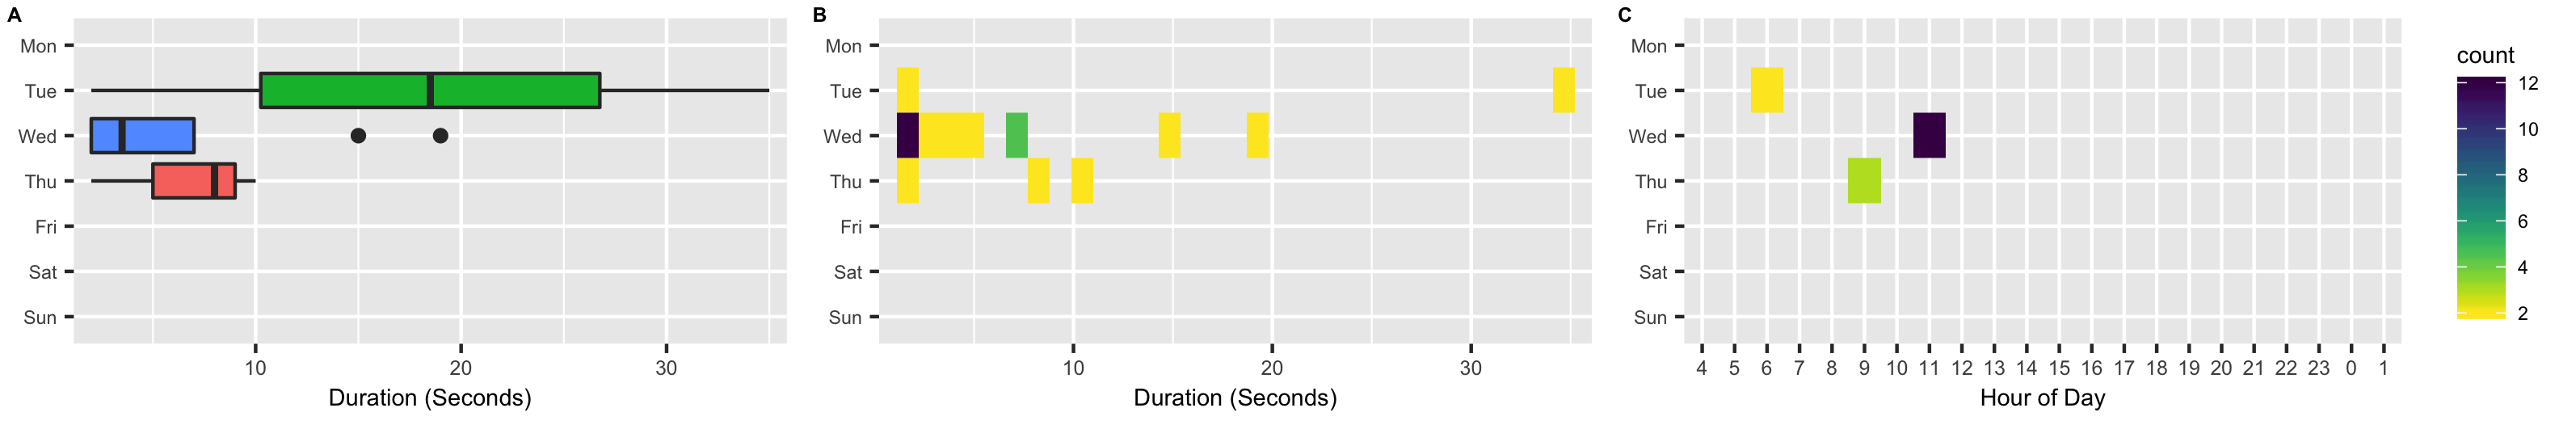
\includegraphics[width=1\linewidth]{/Users/alistairgj/Documents/GitHub/IoT_ResearchProject/IoT_November/images/subAct60} \caption{A caption}\label{fig:pressure}
\end{figure}

\begin{figure}[H]
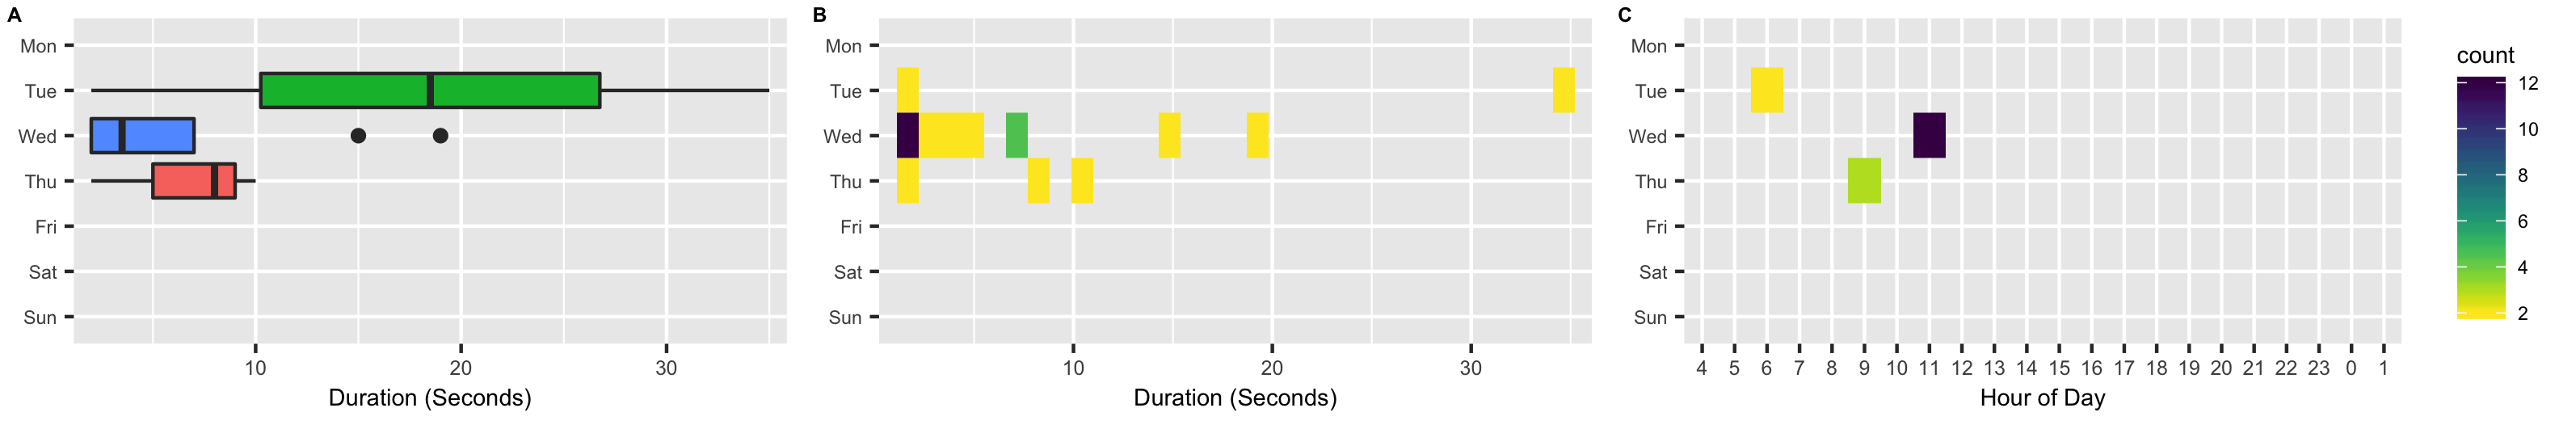
\includegraphics[width=1\linewidth]{/Users/alistairgj/Documents/GitHub/IoT_ResearchProject/IoT_November/images/subAct60} \caption{A caption}\label{fig:pressureFULL}
\end{figure}

\begin{Shaded}
\begin{Highlighting}[]
\OperatorTok{%}\NormalTok{run }\OperatorTok{-}\NormalTok{i reqEnergy_containSpecialCharClean.py}
\end{Highlighting}
\end{Shaded}

Test for in \ref{fig:fig1} we see XYZ

\begin{figure}
\centering
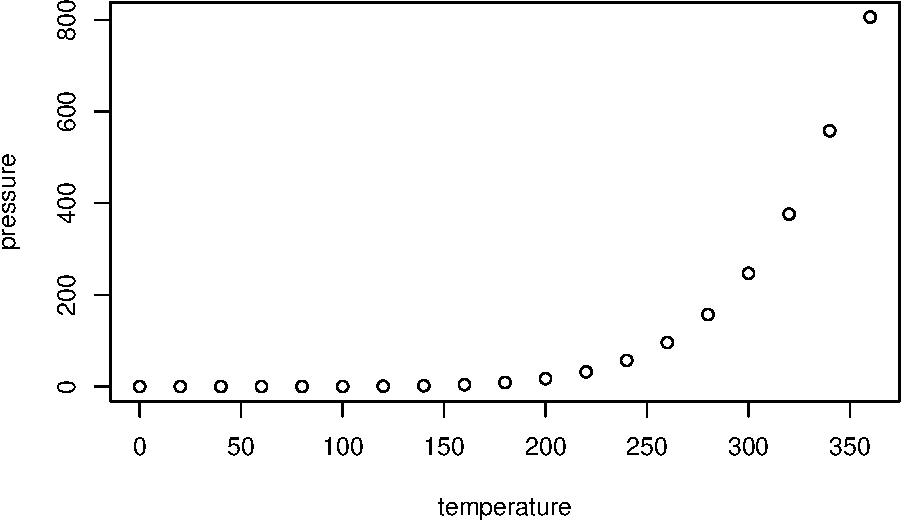
\includegraphics{MD_Final_files/figure-latex/fig1-1.pdf}
\caption{\label{fig:fig1}This is a caption}
\end{figure}

Reduce image border (not working???)
\url{https://holtzy.github.io/Pimp-my-rmd/}


\end{document}
